\documentclass[11pt]{article}
\usepackage[paper=a4paper,left=24mm,right=24mm,top=20mm,bottom=20mm]{geometry}

\usepackage[english]{babel}
\usepackage{amsmath}                                % For textit, textbf, etc
\usepackage{graphicx}                               % For includegraphics
\usepackage{wrapfig}                                % For wrapfig environment
\usepackage{paralist}                               % For compactitem 
\usepackage{hyperref}
\hypersetup{
    colorlinks=true,
    linkcolor=blue,
    %filecolor=magenta,      
    urlcolor=blue,
    %pdftitle={Overleaf Example},
    %pdfpagemode=FullScreen,
    }
\pagestyle{empty}                                   % No pagenumbers/headers/footers

%%% Custom sectioning (sectsty package)
\usepackage{sectsty}
\sectionfont{%			                            % Change font of \section command
	\usefont{OT1}{phv}{m}{n}%		                
	\sectionrule{0pt}{0pt}{-10pt}{1pt}
}
\subsectionfont{%			                        % Change font of \subsection command
	\usefont{OT1}{phv}{m}{n}%		                
	%\sectionrule{0pt}{0pt}{-10pt}{1pt}
}

%%% Macros
\newcommand*{\inlineimg}[1]{%
    \raisebox{-.3\baselineskip}{%
        \includegraphics[
            height=\baselineskip,
            width=\baselineskip,
            keepaspectratio,
        ]{#1}%
    }%
}

\newcommand{\sepspace}{\vspace*{1em}}		        % Vertical space macro
\newcommand{\NewPart}[1]{\section*{\uppercase{#1}}}
\newcommand{\NewSubPart}[1]{\subsection*{#1}}

\newcommand{\MyName}[1]{
    \noindent
	\Huge \usefont{OT1}{phv}{m}{n} #1 \hfill        % Name
	\par \normalsize \normalfont
}

\newcommand{\SimpleEntry}[1]{
	\noindent\hangindent=0.5cm\hangafter=0          % Indentation
	#1 \par                                         % Entry 
}

\newcommand{\TimeEntry}[4]{
    \noindent\hangindent=0.5cm\hangafter=0          % Indentation
    \parbox{3cm}{                                   % Box to align text
	    \textit{#1}                                 % Time
	}
	\textbf{#2}                                     % What
	\text{#3}                                       % Work
	\normalsize \par
}

\newcommand{\TimeEntryFocus}[5]{
    \noindent\hangindent=0.5cm\hangafter=0          % Indentation
    \parbox{3cm}{                                   % Box to align text
	    \textit{#1}                                 % Time
	}
	\textbf{#2}                                     % What
	\text{#3} \par                                  % School
	\noindent\hangindent=3.7cm\hangafter=0
	\textit{#4}                                     % Average, Focus, etc
	\normalsize \par
}

\newcommand{\TimeEntryDesc}[4]{
    \noindent\hangindent=0.5cm\hangafter=0          % Indentation
    \parbox{3cm}{                                   % Box to align text
	    \textit{#1}                                 % Time
	}
	\textbf{#2}                                     % What
	\text{#3} \par                                  % Work
	\noindent\hangindent=4cm\hangafter=0 \parbox{11cm}{\vspace{0.2em}\small #4}  % Description
	\normalsize \par
}

\newcommand{\TimeEntryFocusDesc}[5]{
    \noindent\hangindent=0.5cm\hangafter=0          % Indentation
    \parbox{3cm}{                                   % Box to align text
	    \textit{#1}                                 % Time
	}
	\textbf{#2}                                     % What
	\text{#3} \par                                  % School
	\noindent\hangindent=3.7cm\hangafter=0
	\textit{#4} \par                                  % Average, Focus, etc
	\noindent\hangindent=4cm\hangafter=0 \parbox{12cm}{\vspace{0.2em}\small #5}  % Description
	\normalsize \par
}

\newcommand{\TitleEntry}[2]{                     
	\noindent\hangindent=0.5cm\hangafter=0            % Indentation
	\parbox{3cm}{                                   % Box to align text
	    \textit{#1}
	}			                                    % Title
	#2 \par                                         % Entry	
}

\newcommand{\TitleEntryLong}[2]{                     
	\noindent\hangindent=0.5cm\hangafter=0            % Indentation
	\parbox{14cm}{                                   % Box to align text
	    \textit{#1}
	}			                                    % Title
	#2 \par                                         % Entry	
}


%%% Begin Document
\begin{document}
% \begin{wrapfigure}{r}{0.3\textwidth}
% 	\vspace*{-0.5cm}
%   \hfill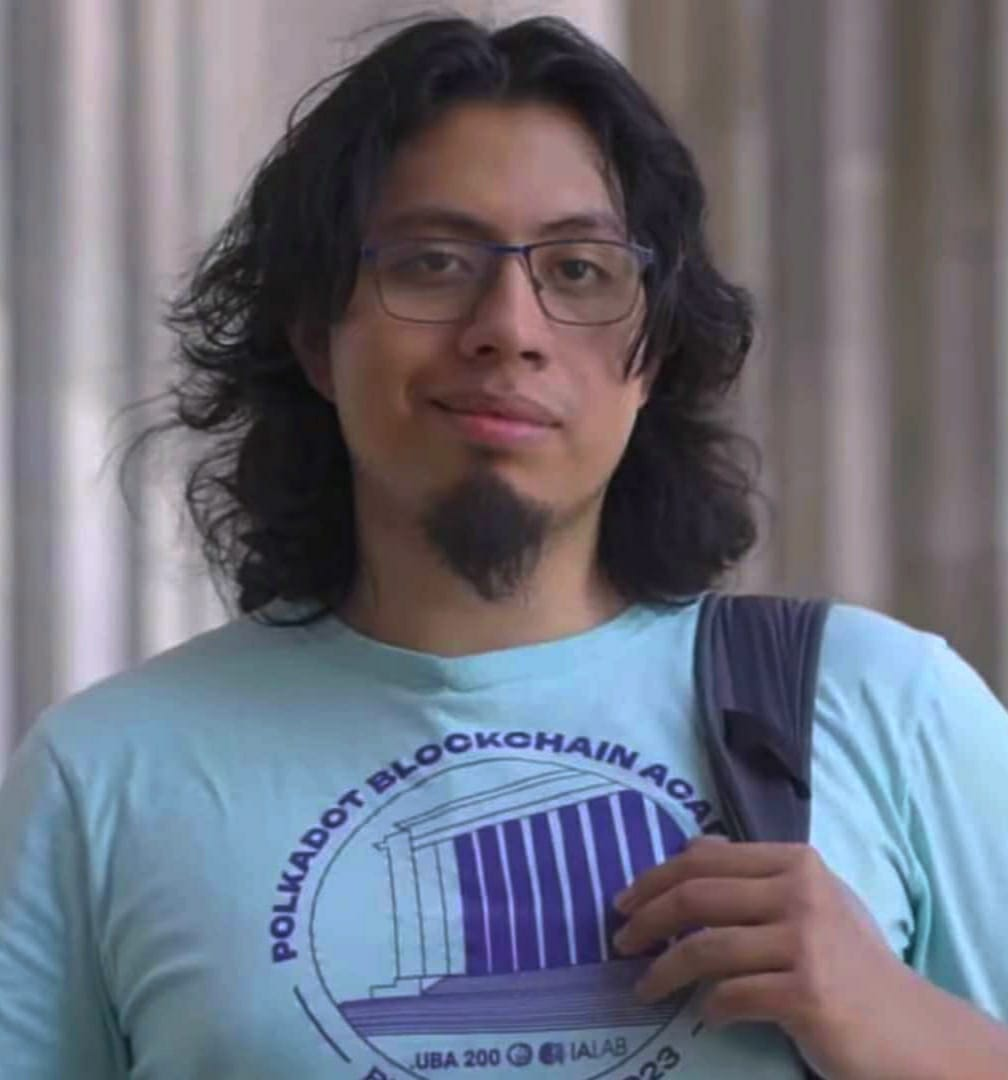
\includegraphics[width=0.2\textwidth]{photo2.jpeg}
% 	\vspace{-5cm}
% \end{wrapfigure}
\MyName{Daniel S\'anchez Dom\'inguez}
\SimpleEntry{\textbf{\Large{Software Engineer}}}
\sepspace

%%% Personal details
%\NewPart{Personal details}

\SimpleEntry{(+52) 811 84 71 700}
\SimpleEntry{\href{mailto:amaniel2718@protonmail.com}{amaniel2718@protonmail.com}}

\NewPart{Professional experience}

\TimeEntryFocus{16.Oct.2023 - Dic.2023}{Automation project for RISTOC}{}
{Project to automate the workflow of an online automotive parts store. The developed
components included: a \textbf{PostgreSQL} database, backend logic implemented in
\textbf{Python}, integration with Shopify and automated workflows using \textbf{Zapier}.}

\TimeEntryFocus{20-23.Sep.2023}{3rd place: Hackaton Cripto México Tijuana}{}
{Developed a functional MVP of a \textbf{Liquidity Stake} over the \textbf{VARA}
network. The \textbf{smart contracts} were programmed in \textbf{Rust}.}

\TimeEntryFocus{17.Aug.2023}{Rust Trainer in a Workshop at CryptoLatin Fest}{: (Colombia)}
{Conducted a workshop targeting developers interested in learning \textbf{Rust}
and writing smart contracts with \textbf{Ink!}.}

\TimeEntryFocus{Jul.2023 - Currently}{CriptoMx Guardian Protocol}{Blockchain Developer}
{Working at the design of smart contracts in \textbf{Rust} to implement a
liquidity staking protocol in the \textbf{VARA} network. }

\TimeEntryFocus{07.Jun.2023}{\inlineimg{icons/Ibero.png} Rust Trainer in a Workshop at Univ. Iberoamericana}{}
{Workshop oriented to university students, focused to teach them solid foundations
on \textbf{Rust} and writing smart contracts with \textbf{Ink!}.}

\TimeEntryFocus{Apr.2023 - ...}{Freelancing projects}{}
{Working to develop a basic cybersecurity toolchain (a Fuzzer and Static
Analyzer) for analyzing vulnerabilities in WASM binaries used in \textbf{Ink!}
smart contracts. Utilizing \textbf{Rust} for the implementation.}

\TimeEntryFocus{15.Jan.2022 - 19.Dec.2022}{\inlineimg{icons/johndeere.png} John Deere}{Embedded Systems Engineer}
{Worked in an Agile team using Linux, Python, C, and ARM.
  Accomplishments include designing and implementing a kernel driver
  for communication between a processor and a microprocessor through UART and the IOP protocol,
  developing a Python CLI app for booting only USBs with verified ISO images in Windows,
  resolved build issues in Jenkins,
  and implementing a module in RTOS to convert CAN to Bluetooth.
  Also taught a series of courses on Rust and its application in embedded systems to engineers on the organization. }

\TimeEntryFocus{Summer 2022}{\inlineimg{icons/abclog.png} ABC Logistica}{Web Developer}
{Contracted to document and implement tests in PHP using the Laravel framework.
  Worked with languages like SQL and JavaScript.}


%%% Education
\NewPart{Education}
\TimeEntryFocus{Jan.2023-Feb.2023}{\inlineimg{icons/Polkadot.png} Polkadot Blockchain Academy}{: \textbf{Parity} x \textbf{UBA} (Argentina)}
{An in deepth course, research oriented, working with core libraries of the \textbf{Substrate} framework in \textbf{Rust}}

\TimeEntryFocus{2018-2022}{\inlineimg{icons/fime.png} University studies as Network Engineer}{: \textbf{UANL} (Mexico)}
{Focused on sistems programming and embedded development}

\TimeEntryFocus{Autumn 2020 - Summer 2021}{\inlineimg{icons/Qiskit-Logo.svg.png} The Coding School’s Qubit by Qubit}{: \textbf{IBM}}
{Completed a two-semester Quantum Computing course using the \textbf{Qiskit} framework}

\TimeEntryFocus{Spring 2022}{\inlineimg{icons/cardano.png} Plutus Pioneers 3rd Cohort}{: \textbf{IOHK}}
{Completed a hands-on course using \textbf{Haskell} to learn about the Cardano Blockchain and Smart Contracts development.}

	%Average to date: 5\\
	%Expected graduation in June of 2024}

\sepspace
%%% Academic Activities
\NewPart{Academic Activities}
% \TimeEntryFocus{02-11.2009}{Piano course}
% {taught by María Isabel García López}{}
 
% \TimeEntryFocus{Autumn.2011}{Mini Robótica para Adolescentes}
% {program taught by ITESO}{}

\TimeEntryFocus{10-22.Nov.2020}{\inlineimg{icons/igem.png} iGEM Competition}{Gold mendal as member of the FCB-UANL team}{
  Modification of a bacterium for the expression of ranaspumins, a thermo-resistant protein, 
  for producing fire-fighting foam.}

\TimeEntryFocus{Summer 2020}{X Escuela de Verano Virtual de Matemáticas}{organized by the \textbf{UNAM}}{
  Focus on numerical methods to model pandemic dynamics using Python}

\TimeEntryFocus{01-04.Nov.2019}{\inlineimg{icons/igem.png} iGEM Competition}{Bronze medal as member of the UANL team}{
Designed genetically engineered bacteria for digesting toxic compounds.
Used Python for numerical simulations and cluster computing.
Created an online wiki to document the project.
Presented the project at the iGEM competition in Boston, USA.}

\TimeEntryFocus{Autumn 2019}{Túnel de la biología sintética}{}{Scientific divulgation activity}

\TimeEntryFocus{Autumn 2019}{Program: CON-CIENCIA UANL}{Participation as organizer}{
  Program to promote STEM skills aimed at low-income high school students.
  Conducted a course on programming concepts and digital electronics.}

\TimeEntryFocus{04-20.Sep.2019}{Course: Biotecnología de Cianobacterias y Microalgas}{: \textbf{FCB-UANL}}
{Hands-on workshop given by MSc. Alejandra Torres Ariño, aimed to learn how to
  extract microalgae, cultivate cyanobacteria and count organisms under a microscope.}

\TimeEntryFocus{Summer 2019}{Course: Biotecnología Aplicada a Biomedicina Molecular}{: \textbf{CIDEB-UANL}}
{Hands-on course given by MSc. Heber Torres Cordero, to learn DNA extraction techniques,
  protein purification, and identification of diseases through molecular techniques.}

\TimeEntryFocus{Feb.2019}{Olimpiada del Conocimiento}{organized by the UANL: 3rd place}{}

\TimeEntryFocus{Sep.2017}{Festival Internacional y Masterclass de Piano}{: \textbf{UANL}}
{Participation as pianist interpeter}

\TimeEntryFocus{Jul.2017}{2º Concurso Nacional de Piano}{: \textbf{Universidad de Guadalajara}}{}

\TimeEntryFocus{30.01.2015}{Concurso Nacional de Jóvenes Pianistas Parnassós}{on the Fourth Level}{}


%%% Skills and Qualifications
\NewPart{Skills and Qualifications}
\NewSubPart{Languages}
\TitleEntry{Native tongue}{Spanish}
\TitleEntry{C1}{English}
\TitleEntry{A2}{French}

\NewSubPart{Programming Languages}
\TitleEntry{Advanced}{\inlineimg{icons/bash.png} Bash/Linux}
\TitleEntry{Advanced}{\inlineimg{icons/python.png} Python}
\TitleEntry{Proeficient}{\inlineimg{icons/rust.png} Rust}
\TitleEntry{Proeficient}{\inlineimg{icons/C_lang.png} C}
\TitleEntry{Intermediate}{\inlineimg{icons/haskell.png} Haskell}
\TitleEntry{Basic Skills}{\inlineimg{icons/laravel.png} PHP/Laravel}

%%% Links of interest
\NewPart{Links of interest}
\TitleEntry{\inlineimg{icons/github.png} Github}{\href{https://github.com/DanEscher98}{DanEscher98}}
\TitleEntry{\inlineimg{icons/linkedin.png} LinkedIn}{\href{https://www.linkedin.com/in/danyiel-colin}{Danyiel Colin}}
\TitleEntry{\inlineimg{icons/devto.png} Dev.to}{\href{https://dev.to/danescher98}{Technical blog}}
\TitleEntry{\inlineimg{icons/igem.png} iGEM project}{\href{https://2019.igem.org/Team:UANL}{iGEM UANL 2019}}
\TitleEntry{\inlineimg{icons/igem.png} iGEM project}{\href{https://2020.igem.org/Team:FCB-UANL}{iGEM FCB-UANL 2020}}
\TitleEntry{\inlineimg{icons/youtube.png} Workshop}{\href{https://www.youtube.com/live/ikxfT709f3k?feature=share&t=1h56m}{Youtube} Rust Workshop in Spanish}


\end{document}
